% Standalone source of the massless three-vertex chain used in the regulator
% application example of Sec. 5 of the paper. Drawing conventions follow the dS
% Feynman rules of the dSIBP paper (figures fig_skrules/fig_linetypes): black
% vertices sit on the + branch, external legs end on the white squares of the
% boundary insertions, and internal propagators are directed straight lines
% whose arrows mark the momentum flow (the single-propagator style of
% fig_linetypes; arcs are only needed when two propagators share one vertex
% pair as in the bubble of fig_skrules).
% Compile: pdflatex fig_ep_tree.tex   (produces fig_ep_tree.pdf, included by paper.tex)
\documentclass[tikz,border=6pt]{standalone}
\usetikzlibrary{calc}
\begin{document}
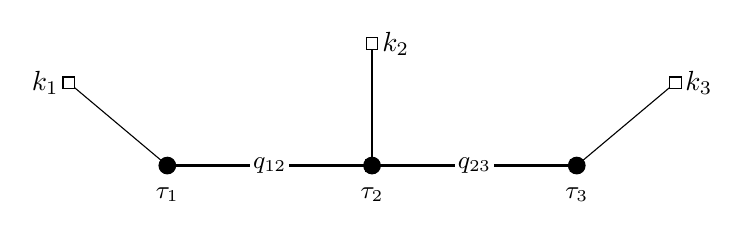
\begin{tikzpicture}[every node/.style={inner sep=1.5pt}]
  % Three time vertices on the + branch, left to right v = 1, 2, 3.
  \coordinate (v1) at (0,0);
  \coordinate (v2) at (2.6,0);
  \coordinate (v3) at (5.2,0);
  % External legs, one per vertex, ending on the boundary squares.
  \draw (v1) -- (-1.25,1.05);
  \draw (v2) -- (2.6,1.55);
  \draw (v3) -- (6.45,1.05);
  \filldraw[fill=white,draw=black] ($(-1.25,1.05)+(-0.075,0.075)$) rectangle ++(0.15,-0.15);
  \filldraw[fill=white,draw=black] ($(2.6,1.55)+(-0.075,0.075)$) rectangle ++(0.15,-0.15);
  \filldraw[fill=white,draw=black] ($(6.45,1.05)+(-0.075,0.075)$) rectangle ++(0.15,-0.15);
  \node[left=2pt]  at (-1.25,1.05) {$k_1$};
  \node[right=2pt] at (2.6,1.55)   {$k_2$};
  \node[right=2pt] at (6.45,1.05)  {$k_3$};
  % The two internal massless full propagators: directed straight lines,
  % arrows marking the momentum flow of magnitudes q_{12} and q_{23}.
  \draw[->,thick] (v1) -- (v2);
  \draw[->,thick] (v2) -- (v3);
  \node[fill=white,inner sep=1pt] at (1.3,0)  {\small $q_{12}$};
  \node[fill=white,inner sep=1pt] at (3.9,0)  {\small $q_{23}$};
  % Vertex times below the vertices, clear of the propagator lines.
  \node[anchor=north] at (0,-0.22)   {\small $\tau_1$};
  \node[anchor=north] at (2.6,-0.22) {\small $\tau_2$};
  \node[anchor=north] at (5.2,-0.22) {\small $\tau_3$};
  % Vertices last.
  \filldraw[fill=black,draw=black] (v1) circle (3pt);
  \filldraw[fill=black,draw=black] (v2) circle (3pt);
  \filldraw[fill=black,draw=black] (v3) circle (3pt);
\end{tikzpicture}
\end{document}
